\chapter{\label{ch:experimentandresult}Experiments and results}
In this chapter a comparison of wavelets discussed in chapter  \ref{ch:wavelets} is analyzed with characteristic scenes in 2D (flatland) and 3D. Such a comparison can never be exhaustive due to the heterogeneous nature of input scenes. Therefore scenes with different kind of kernels has been chosen for comparison of performance of the wavelets. We first discuss kernels for which we have the exact analytical solution of the integral equation. Then we test and compare the wavelets the 2D scenes knows as flatland scenes. Flatland scenes are selected mainly to analysis and understanding different aspects of using wavelet basis for radiosity. Results of using the different wavelets with 3D scenes are also discussed at the end this chapter. \\

% {\bf Ground truth comparison}\\
\section{Integral Equation with degenerate kernel}
For comparing the approximate solution with exact ground truth we chose kernels which are classified as degenerate kernels. Degenerate kernels are kernels which can be expanded in the form shown in Equation (\ref{eq:kxydegen})
\begin{equation} \label{eq:kxydegen}
K(x,y) = \sum\limits_{i=1}^na_i(x)b_i(y) \\ 
\end{equation}
An integral equation with degenerate kernel can be solved by changing the order of integral and summation after substituting expanded kernel. See a
Appendix \ref{apen:derivationdegenerate} for analytical solution of non-homogeneous Fredholm IE of second kind. 

We took kernel 
\begin{equation}\label{eq:kernelanalytical}
 K(x,y)=x^2+xy, \quad x,y \in [0,1]
\end{equation}
for comparing different wavelets with the ground truth solution 
\begin{equation}\label{eq:solutinoanalytical}
    B(x)=\frac{66}{23}x^2+\frac{42}{23}x+1
\end{equation}
 of the IE shown in Equation \ref{eq:genrie}
 We substitute this kernel in Equation \ref{eq:genrie} to get IE equation,
\begin{eqnarray} \label{eq:analytical}
B(x)=E(x)+\int\limits_0^1 K(x,y)B(y) dy \\
 = E(x)+\int\limits_0^1 (x^2+xy )B(y) dy
\end{eqnarray}

We compare wavelets by calculating error in the projection of kernel $K(x,y)$ and error in solution $B(x)$. The metric used for comparison is relative error as shown in Equation \ref{eq:Krelerr}. It is a ratio of $L^2$ norm of error $(K(x,y)-\hat{K}(x,y))$ to $L^2$ norm of kernel. The integration is over entire domain of x and y. Where $\hat{K}(x,y)$ is approximation of $K(x,y)$ in space spanned by chosen wavelet.
\begin{equation} \label{eq:Krelerr}
\text{relative  error}=\frac{\int\int \,(\,K(x,y)-\hat{K}(x,y)\,)^2  \,dy \, dx}{\int\int \,K(x,y)^2  \,dy \, dx}
\end{equation}
The purpose of selecting degenerate kernel is to make sure that the implemented algorithm works properly and algorithm is fit for testing the wavelets with the scenes for which we do not have the ground truth analytical solution. Note that the kernels discussed in this section does not describe any real world scene. 

Approximate solution is calculate using projection method shown in Chapter \ref{ch:waveletprojection}. Figure \ref{fig:ahaar4}, \ref{fig:ahaar4}, \ref{fig:allmw2}, \ref{fig:allmw4}, \ref{fig:aqlmw2}, shows the approximate solution and error function with different wavelets without thresholding(replacing negligible elements  with value 0). This shows that as we increase n, error reduces and as we increase vanishing moments of wavelet from Haar wavelet to QLMW error decreases. Above two result shows that to decrease error in  solution either n or order basis function has to be increased. Also for QLMW error is zero for all $n$ because $K(x,y)$ lies in space spanned by QLMW basis.



\begin{figure}[h!]
\centering{}
\captionsetup{justification=centering}
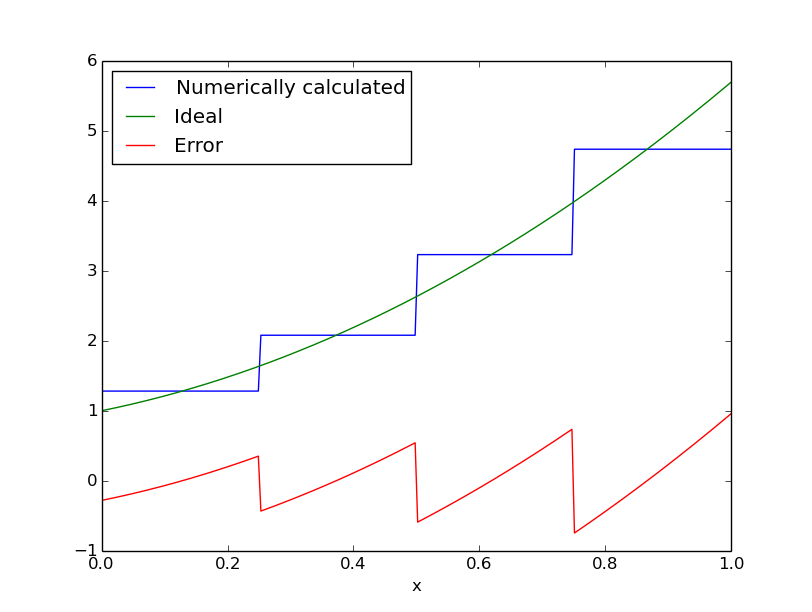
\includegraphics[width=5in]{ahaar4.png}
\caption{\label{fig:ahaar4}Haar wavelet: Solution and Error in solution of Equation \ref{eq:analytical} with $n=4$}
\end{figure}

\begin{figure}[h!]
\centering{}
\captionsetup{justification=centering}
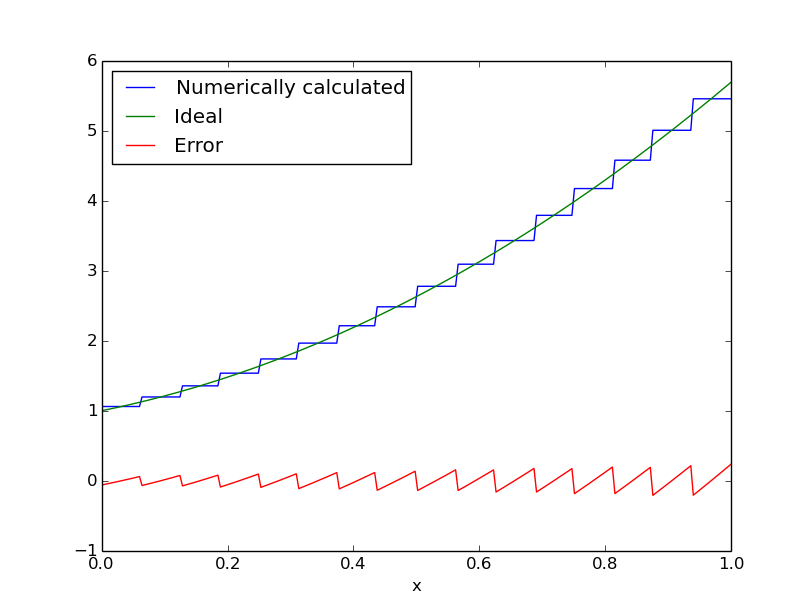
\includegraphics[width=5in]{ahaar16.png}
\caption{\label{fig:ahaar16}Haar wavelet: Solution and Error in solution of Equation \ref{eq:analytical} with $n=16$}
\end{figure}
\begin{figure}[h!]
\centering{}
\captionsetup{justification=centering}
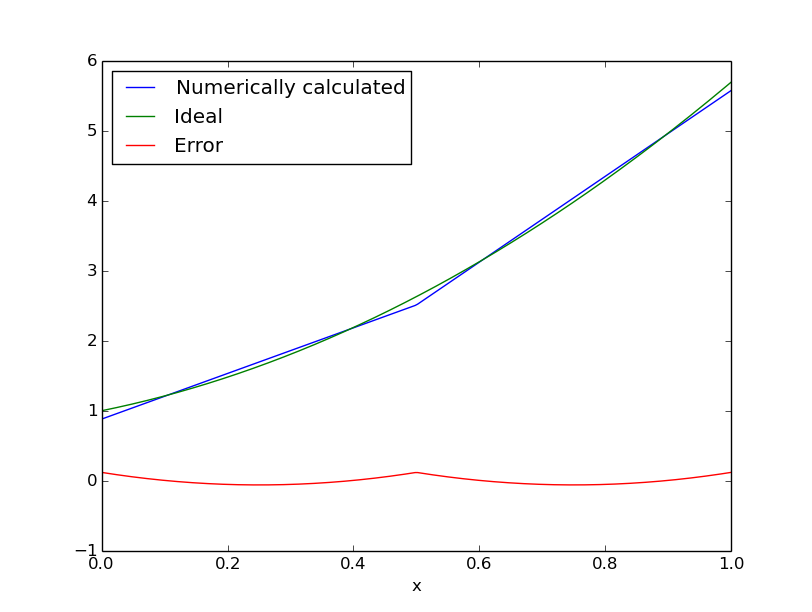
\includegraphics[width=5in]{allmw2.png}
\caption{\label{fig:allmw2}LLMW wavelet: Solution and Error in solution of Equation \ref{eq:analytical} with $n=2$}
\end{figure}
\begin{figure}[h!]
\centering{}
\captionsetup{justification=centering}
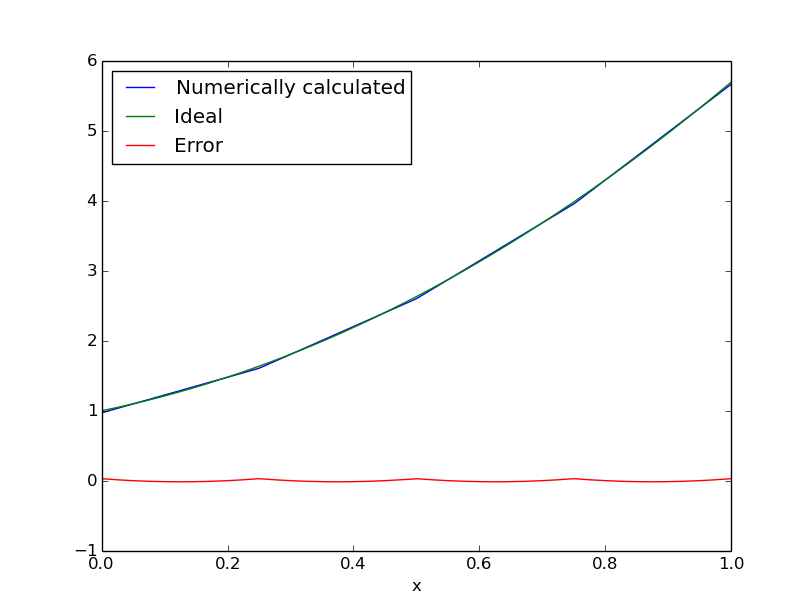
\includegraphics[width=5in]{allmw4.png}
\caption{\label{fig:allmw4}LLMW wavelet: Solution and Error in solution of Equation \ref{eq:analytical} with $n=4$}
\end{figure}


\begin{figure}[h!]
\centering{}
\captionsetup{justification=centering}
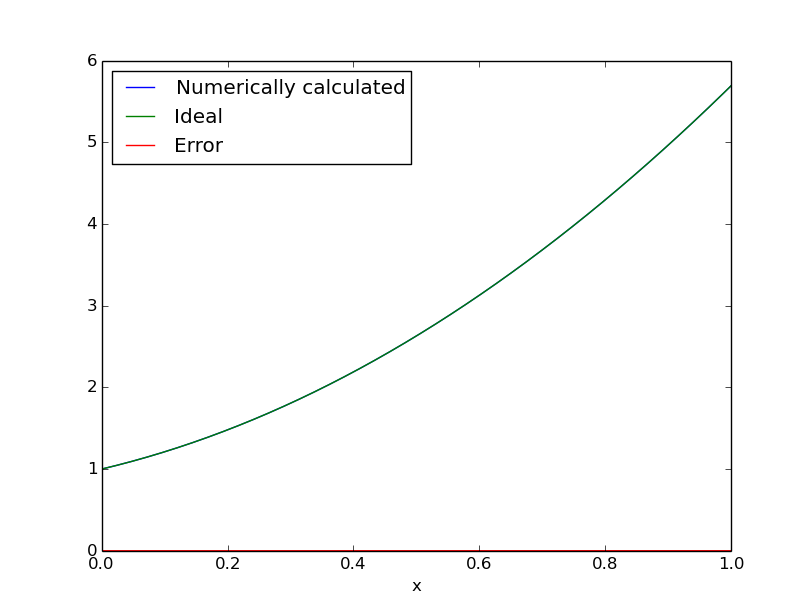
\includegraphics[width=5in]{aqlmw2.png}
\caption{\label{fig:aqlmw2}QLMW wavelet: Solution and Error in solution of Equation \ref{eq:analytical} with $n=2$}
\end{figure}

As we have tested implemented algorithm with 2D kernels, we also have tested algorithm with 4D kernels as shown below,
\begin{equation}\label{eq:kernelanalytical4d}
 K(x_1,y_1,x_2,y_2)=x_1 y_1 x_2 y_2, \quad x_1,y_1,x_2,y_2 \in [0,1]
\end{equation}
The analytical solution \ref{apen:derivationdegenerate} of the integral equation with above kernel,
\begin{eqnarray} \label{eq:analytical4d}
B(x_1,y_1)=E(x_1,y_1)+\int\limits_0^1 K(x_1,y_1,x_2,y_2)B(x_2,y_2) dy \\
 = E(x_1,y_1)+\int\limits_0^1 (x_1y_1x_2y_2)B(x_2,y_2) dy
\end{eqnarray}
is,
\begin{equation}\label{eq:solutinoanalytical4d}
    B(x_1,y_1)=1+\frac{9}{32}x_1y_1
\end{equation}

The comparison of different wavelet is done in similar way as in 2D kernel case seen above. Figure \ref{fig:4d_analytical_haar_2}, \ref{fig:4d_analytical_llmw_2} and \ref{fig:4d_analytical_qlmw_2} shows the comparison of solution with $m=0,1,2$ and $n=2$. Note that numerical solution with $m=1,2$ is same as analytical solution as the approximate finite space is same as the space of original problem. Figure \ref{fig:4d_analytical_haar_4} shows the solution with $m-0$ and $n=4$. 

\begin{figure}[h!]
\centering{}
\captionsetup{justification=centering}
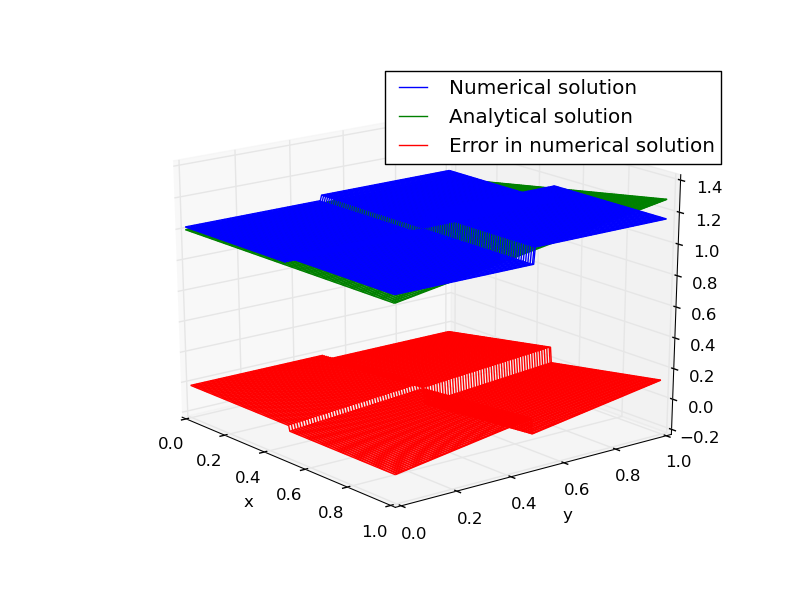
\includegraphics[width=5in]{4d_analytical_haar_2.png}
\caption{\label{fig:4d_analytical_haar_2}Haar wavelet: Analytical and Numerical solution of equation \ref{eq:analytical4d} with $n=2$}
\end{figure}



\begin{figure}[h!]
\centering{}
\captionsetup{justification=centering}
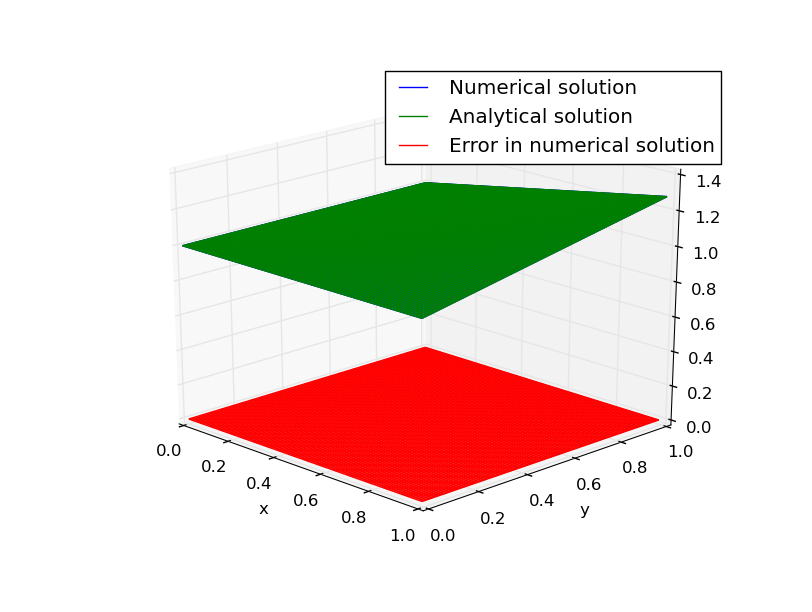
\includegraphics[width=5in]{4d_analytical_llmw_2.png}
\caption{\label{fig:4d_analytical_llmw_2}LLMW wavelet: Analytical and Numerical solution of equation \ref{eq:analytical4d} with $n=2$}
\end{figure}


\begin{figure}[h!]
\centering{}
\captionsetup{justification=centering}
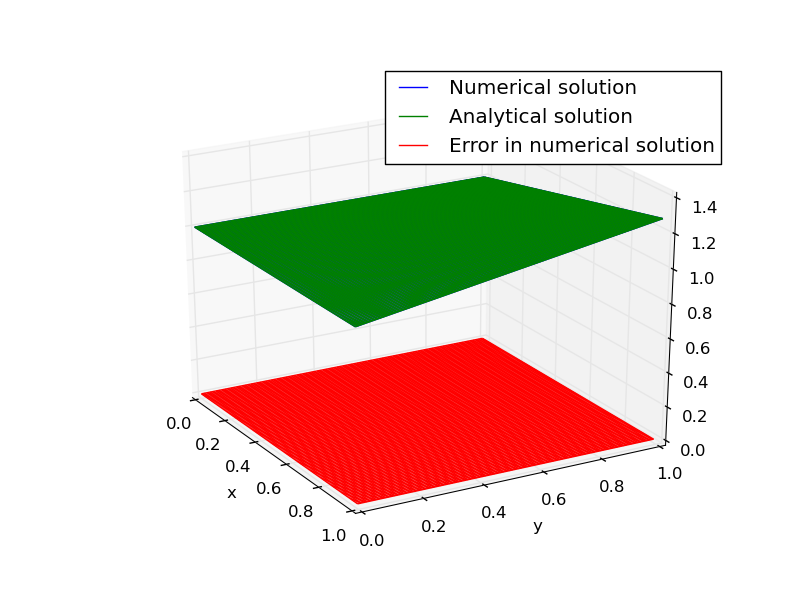
\includegraphics[width=5in]{4d_analytical_qlmw_2.png}
\caption{\label{fig:4d_analytical_qlmw_2}QLMW wavelet: Analytical and Numerical solution of equation \ref{eq:analytical4d} with $n=2$}
\end{figure}

\begin{figure}[h!]
\centering{}
\captionsetup{justification=centering}
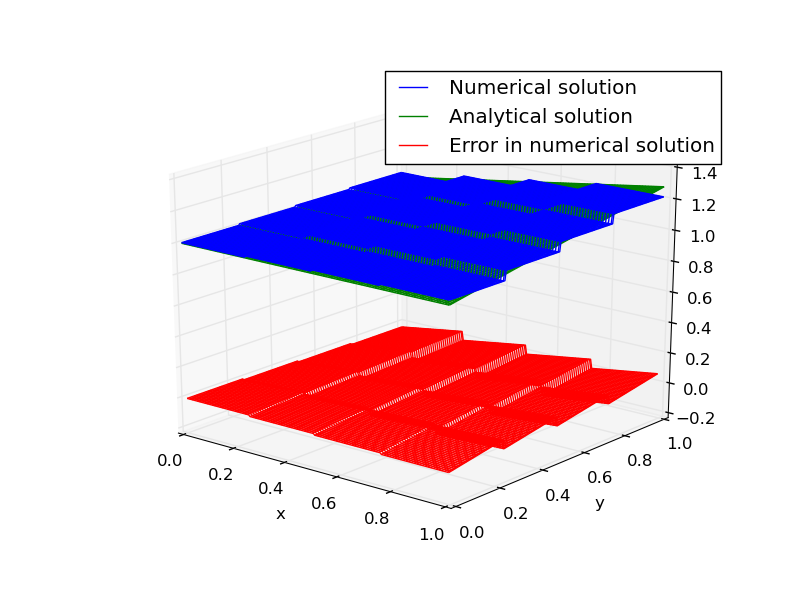
\includegraphics[width=5in]{4d_analytical_haar_4.png}
\caption{\label{fig:4d_analytical_haar_4}Haar wavelet: Analytical and Numerical solution of equation \ref{eq:analytical4d} with $n=4$}
\end{figure}


\section{Flatland radiosity}
In this section we first discuss the relation of $n$ and $m$ with accuracy of projection of kernel for flatland scenes.  Then we discuss the comparison of different wavelets to solve radiosity for flatland scenes. Flatland is two dimensional world in which surfaces are one dimensional instead of two dimensional surfaces in three dimensional scene. We select flatland scenes for its simplicity and imaginability of kernel associated with scenes. Simplest flatland scene is scene with two parallel line segment of unit length each(see Figure \ref{fig:f1scene}) and scene with two line segment, of unit length each, perpendicular to each other(see Figure \ref{fig:f2scene}). 



Note that $x \in X$ and $y \in Y$ in above kernels. $K(x_1,x_2) = 0$ for $x_1,x_2 \in X$ as two points in a line segment do not interact directly, however they can interact indirectly through reflections from other line segment(see Figure \ref{fig:kernel}) for graphical representation of kernel of any two line segment in general. In other words interaction can take place only between two different planner surfaces(on lines in this context) on however, two points on single concave surface(or line) can interact directly.  The kernel $K(x,y)$ of flatland is calculated using \ref{eq:kernelflatland1}. We will refer to scene consist of parallel line segment as Flatland scene 1 and scene with two perpendicular line segment as Flatland scene 2. Kernel $K_1(x,y)$ for Flatland scene 1 is


\begin{figure}[tbh]
\centering{}
\captionsetup{justification=centering}
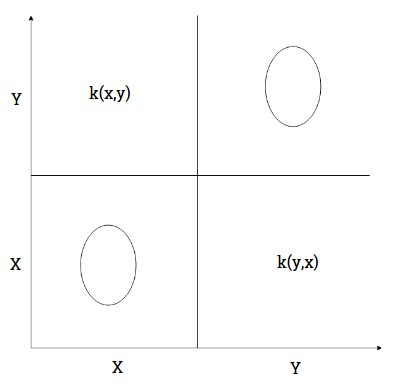
\includegraphics[width=5in]{kernel.png}
\caption{\label{fig:kernel}Flatland scene with two segments: Kernel, in general, with zero and non zero regions}
\end{figure}


\begin{eqnarray} \label{eq:kernelflatland1}
K_1(x,y)\quad=\frac{   \cos{\theta_x}  \cos{\theta_y}  }{    2\,r_{x,y}   }\quad\quad\quad\\
        =\frac{dist^2}{2((x-y)^2+dist^2)}
\end{eqnarray}
and kernel  $K_2(x,y)$ for flatland2 is

\begin{eqnarray} \label{eq:kernelflatland2}
K_2(x,y)\quad=\frac{\cos{\theta_x}\cos{\theta_y}}{2\,r_{x,y}} \quad\quad\quad\quad\quad\quad\quad\quad\quad\quad\\
\quad\quad\quad\quad\quad\quad\quad\quad\quad\quad\quad=\frac{(x+0.1)(y+0.1)}{2((x+0.1)^2+(y+0.1)^2)^{\frac{3}{2}}}\quad\quad\quad
\end{eqnarray}
We can change distance between two line segment in Flatland scene 1 to get different scene. As the distance decrease interaction between two segment increases. Figure \ref{fig:haarscalesparsef1} and \ref{fig:haarwaveletsparsef1} shows the kernel of Flatland scene 1 with $dist=0.25$. The kernel is non negative over entire domain. Also the interaction between two points is maximum when distance between them is less. \\

To see the relation of $n$ and $m$ with accuracy of projection of kernel for flatland scenes we select $m = 0,1,2$ and $n=4,8,16,32,64,128,256$. Figure  \ref{fig:nmtrend_f1} and \ref{fig:nmtrend_f2} conforms the relation of accuracy and n,m for flatland scenes.


\begin{figure}[tbh]
\centering{}
\captionsetup{justification=centering}
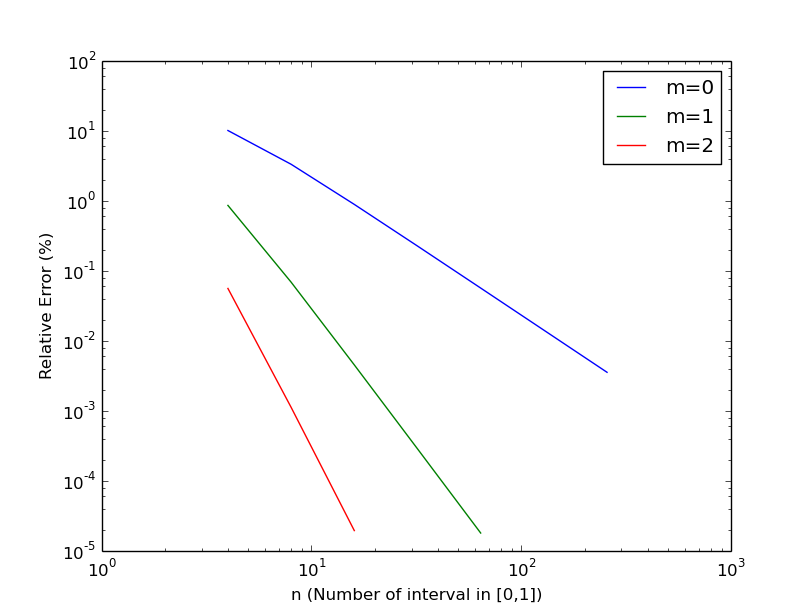
\includegraphics[width=5in]{nmtrend_f1.png}
\caption{\label{fig:nmtrend_f1}Relation of accuracy and n,m in projection of K(x,y) for Flatland Scene 1}
\end{figure}
\begin{figure}[tbh]
\centering{}
\captionsetup{justification=centering}
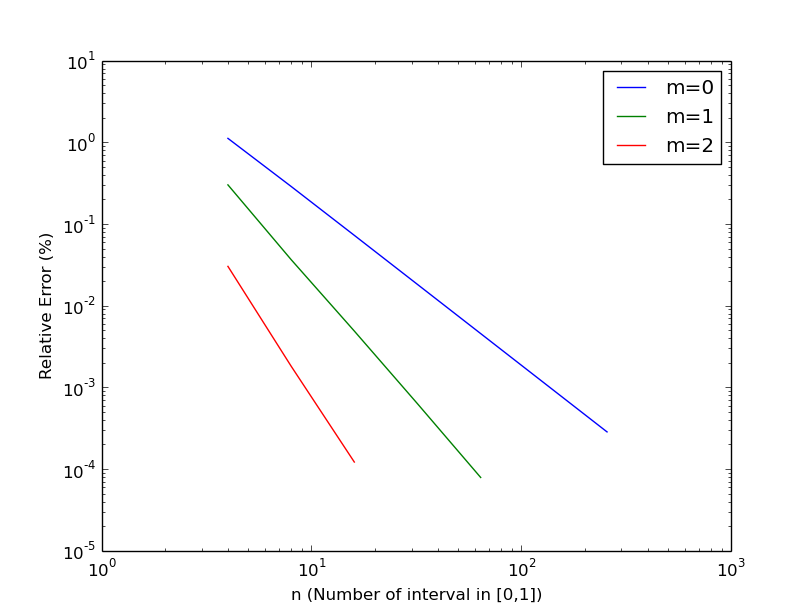
\includegraphics[width=5in]{nmtrend_f2.png}
\caption{\label{fig:nmtrend_f2}Relation of accuracy and n,m in projection of K(x,y) for Flatland Scene 2}
\end{figure}


Kernel is projected into space spanned by wavelet basis to get the sparse matrix of coefficient as shown in \ref{fig:haarwaveletsparsef1} \ref{fig:haarwaveletsparsef2}.




To see the sparsity of matrix we plot sorted elements of matrix. Figure \ref{fig:f1_0_25_haar_scale_distri_n_16} shows that coefficients of Haar wavelet basis are negligible for many basis functions as compared to Haar scaling functions. Similar result for LLMW and QLMW are shown in Figures \ref{fig:f1_0_25_llmw_scale_distri_n_16}, \ref{fig:f1_llmw_scale_distri_n_16}, \ref{fig:f1_0_25_qlmw_scale_distri_n_16}, \ref{fig:f1_qlmw_scale_distri_n_16}.
% {\bf show all the distance and and f2 comment on increase in element value vs decrease in distance also show poly-poly and wavelet-poly comparison for conclusion purpose }

      









\begin{figure}[tbh]
\centering{}
\captionsetup{justification=centering}
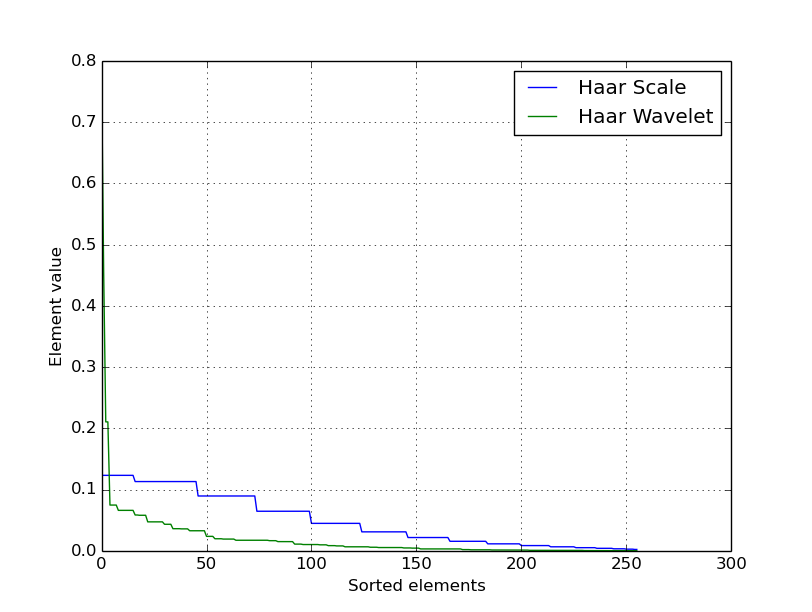
\includegraphics[width=5in]{f1_0_25_haar_scale_distri_n_16.png}
\caption{\label{fig:f1_0_25_haar_scale_distri_n_16}Distribution of kernel projection coefficients with Haar Wavelet and scale functions,$n=16$, for Flatland scene 1}
\end{figure}

\begin{figure}[tbh]
\centering{}
\captionsetup{justification=centering}
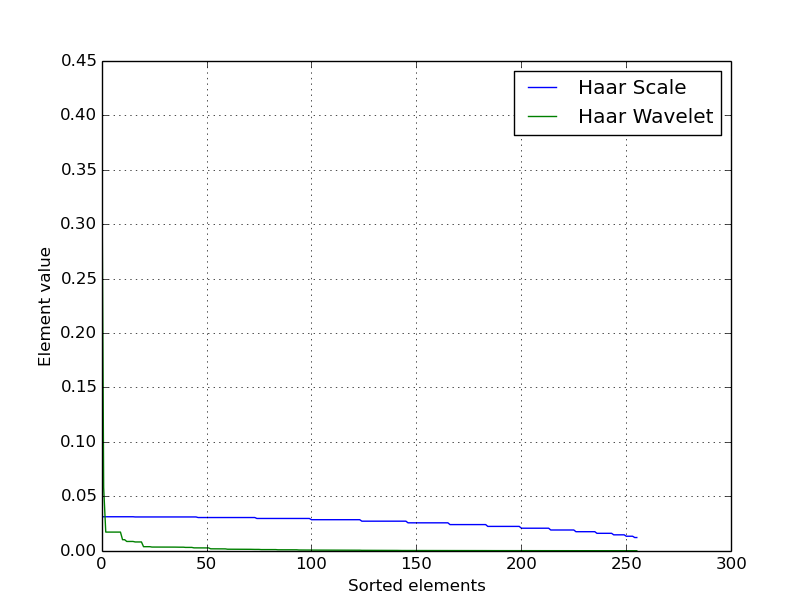
\includegraphics[width=5in]{f1_haar_scale_distri_n_16.png}
\caption{\label{fig:f1_haar_scale_distri_n_16}Distribution of kernel projection coefficients with Haar Wavelet and scale functions,$n=16$, for  Flatland scene 2}
\end{figure}

\begin{figure}[tbh]
\centering{}
\captionsetup{justification=centering}
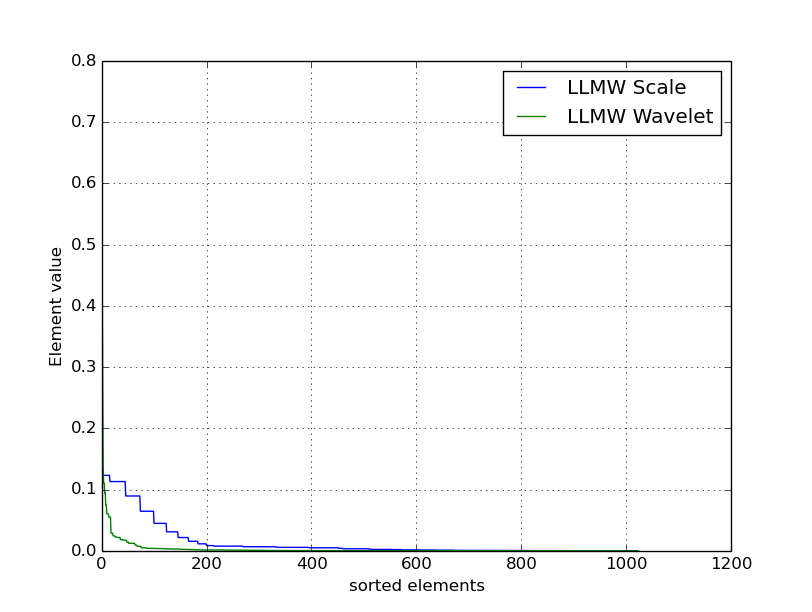
\includegraphics[width=5in]{f1_0_25_llmw_scale_distri_n_16.png}
\caption{\label{fig:f1_0_25_llmw_scale_distri_n_16}Distribution of kernel projection coefficients with LLMW Wavelet and scale functions,$n=16$, for Flatland scene 1}
\end{figure}

\begin{figure}[tbh]
\centering{}
\captionsetup{justification=centering}
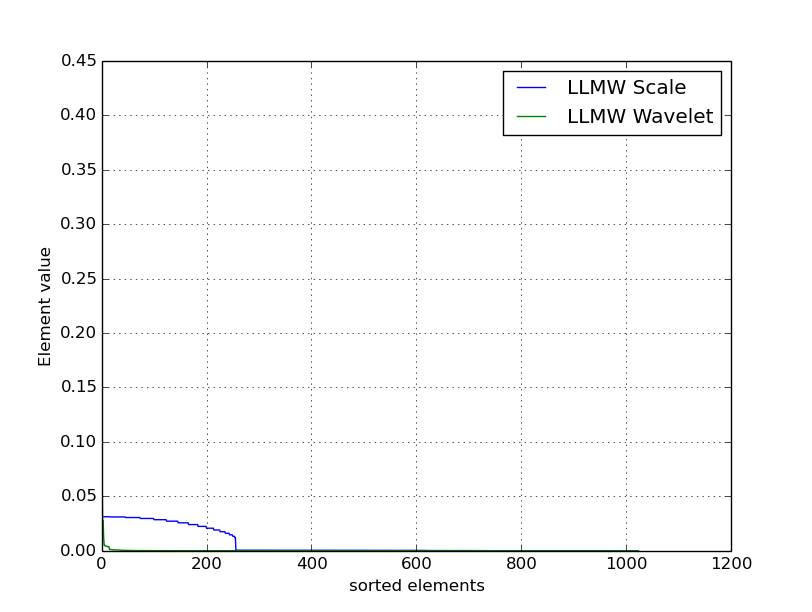
\includegraphics[width=5in]{f1_llmw_scale_distri_n_16.png}
\caption{\label{fig:f1_llmw_scale_distri_n_16}Distribution of kernel projection coefficients with LLMW Wavelet and scale functions,$n=16$, for  Flatland scene 2}
\end{figure}

\begin{figure}[tbh]
\centering{}
\captionsetup{justification=centering}
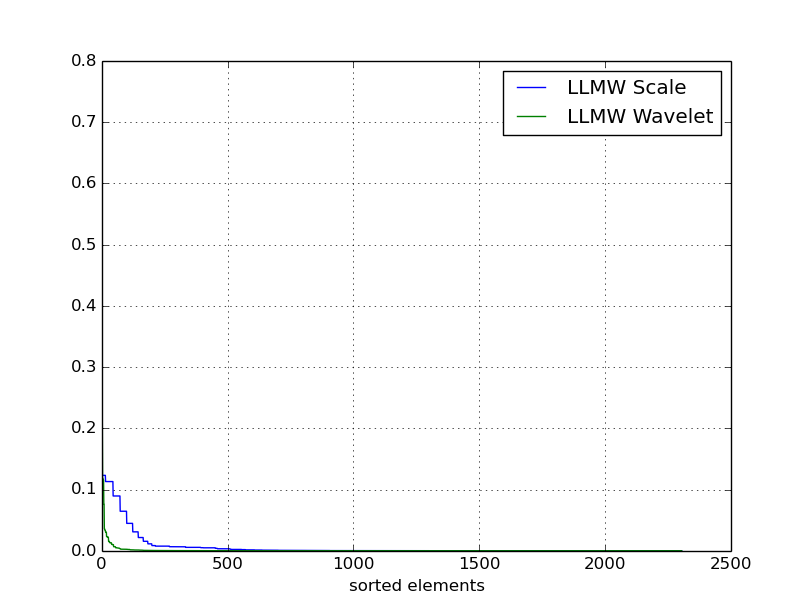
\includegraphics[width=5in]{f1_0_25_qlmw_scale_distri_n_16.png}
\caption{\label{fig:f1_0_25_qlmw_scale_distri_n_16}Distribution of kernel projection coefficients with QLMW Wavelet and scale functions,$n=16$, for Flatland scene 1}
\end{figure}

\begin{figure}[tbh]
\centering{}
\captionsetup{justification=centering}
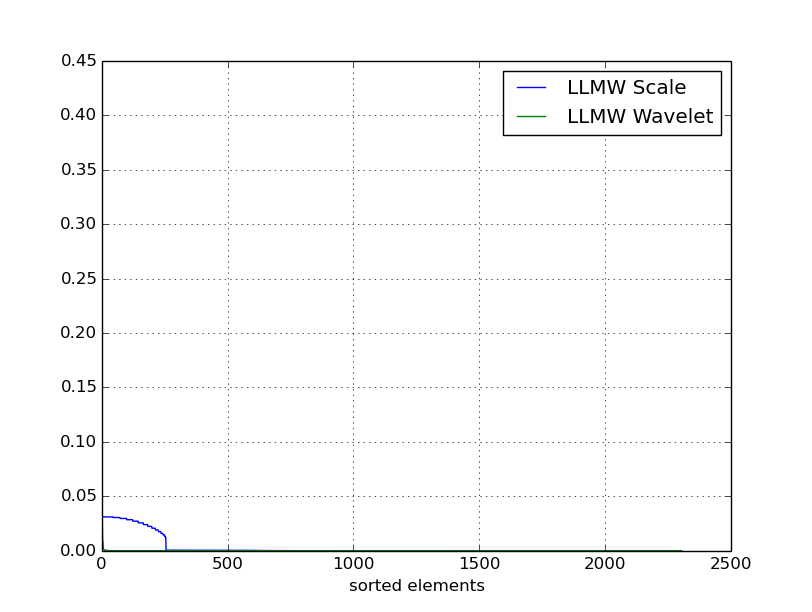
\includegraphics[width=5in]{f1_qlmw_scale_distri_n_16.png}
\caption{\label{fig:f1_qlmw_scale_distri_n_16}Distribution of kernel projection coefficients with QLMW Wavelet and scale functions,$n=16$, for  Flatland scene 2}
\end{figure}
Now we analyze the effect of setting all this negligible coefficients to zero by projecting kernel of Flatland scene 1 with Haar wavelet and scale basis with $n=256$. We select top $N$ elements from kernel projection while remaining are set to zero (thresholding). Figure \ref{fig:errorvstopnhaarwavelet}, \ref{fig:errorvstopnllmwwavelet} shows that error in projection of kernel after thresholding is much less in wavelet basis as compared to scaling function basis.


\begin{figure}[tbh]
\centering{}
\captionsetup{justification=centering}
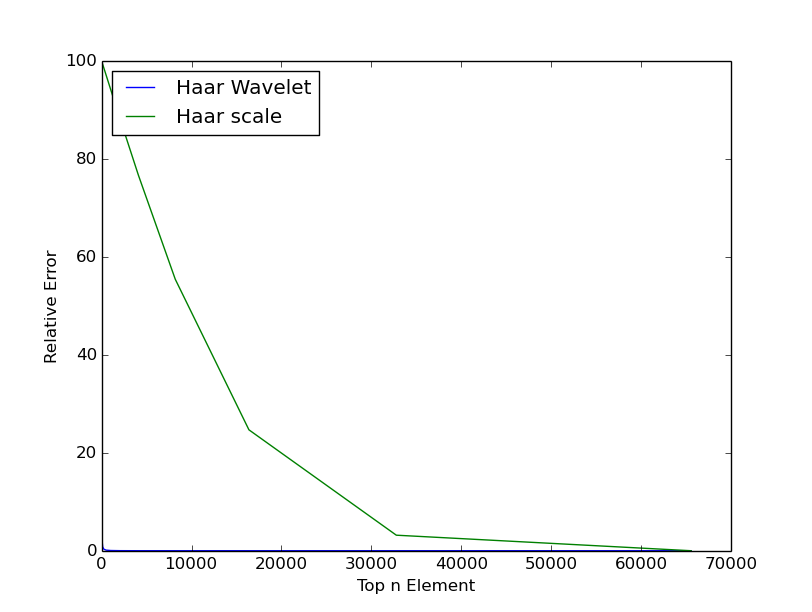
\includegraphics[width=5in]{topn256haarbothf1.png}
\caption{\label{fig:errorvstopnhaarwavelet}Error in projection,  keeping top $N$ element (set remaining to $0$) using both Haar Wavelet and Scale function with $n=256$ for  Flatland scene 1}
\end{figure}

\begin{figure}[tbh]
\centering{}
\captionsetup{justification=centering}
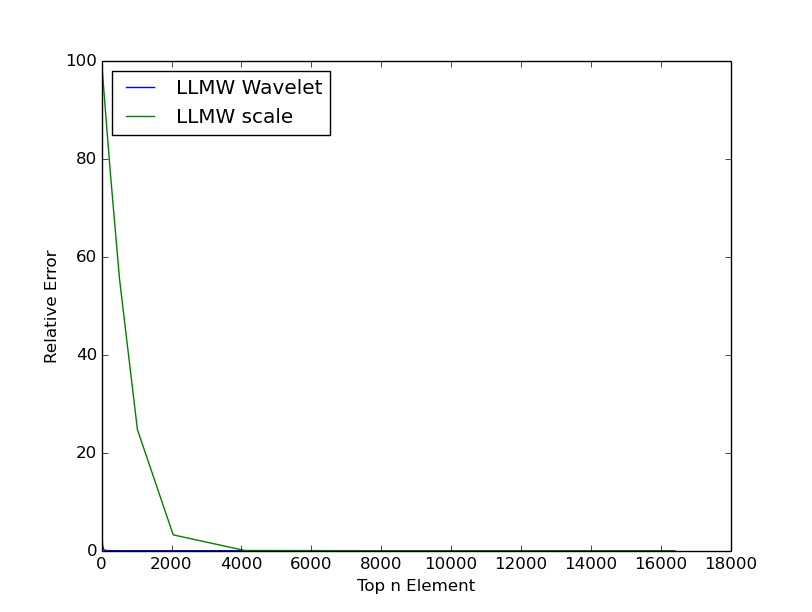
\includegraphics[width=5in]{64topnllmwf1.png}
\caption{\label{fig:errorvstopnllmwwavelet}Error in projection,  keeping top $N$ element (set remaining to $0$) using both LLMW Wavelet and Scale function with $n=64$ for  Flatland scene 1}
\end{figure}

% \begin{eqnarray} \label{eq:kernelflatland1}
% 

% \end{eqnarray}

% \begin{eqnarray} \label{eq:kernelflatland1}
% K_1(x,y)=\frac{\cos{\theta_x}\cos{\theta_y}}{2\,r_{x,y}}\\
% =\frac{dist^2}{2((x-y)^2+dist^2)}

% \end{eqnarray}

% and kernel  $K_2{x,y}$ for flatland2 is


% \begin{eqnarray} \label{eq:kernelflatland2}
% K_1(x,y)=\frac{\cos{\theta_x}\cos{\theta_y}}{2\,r_{x,y}} \quad x,y \in [0,1]
% \end{eqnarray}

Figure \ref{fig:f1_025_haar_scale_plot_n_16}, \ref{fig:f1_025_haar_scale_plot_n_16} and \ref{fig:f1_025_haar_scale_plot_n_16} shows the solution of flatland scene 1 with different $m=0,1,2$ and $n=16$.  We can see that $m=0$ gives blocky solution while $m=1,2$ gives relatively smooth solution.

\begin{figure}%
    \centering
    \subfloat[f1 025 haar scale b1 plot n 16]{{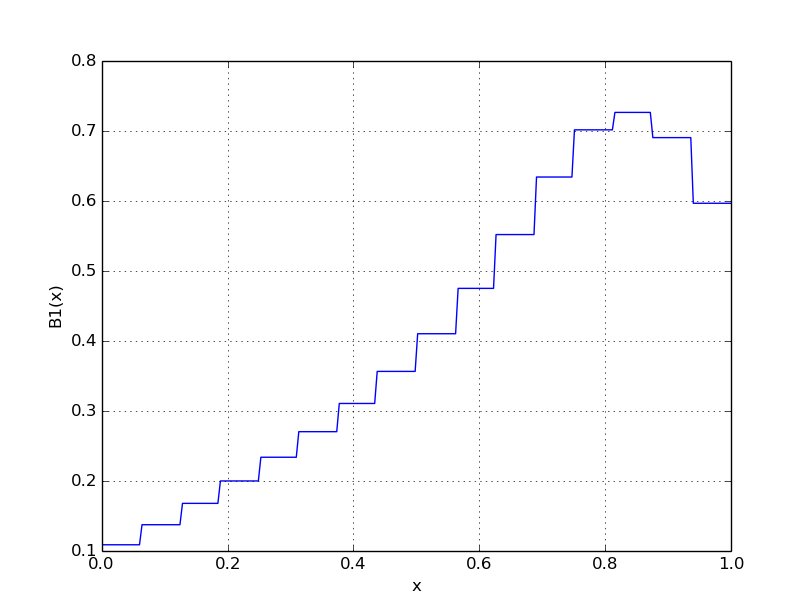
\includegraphics[width=6cm]{f1_025_haar_scale_b1_plot_n_16.png} }}%
    \qquad
    \subfloat[f1 025 haar scale b2 plot n 16]{{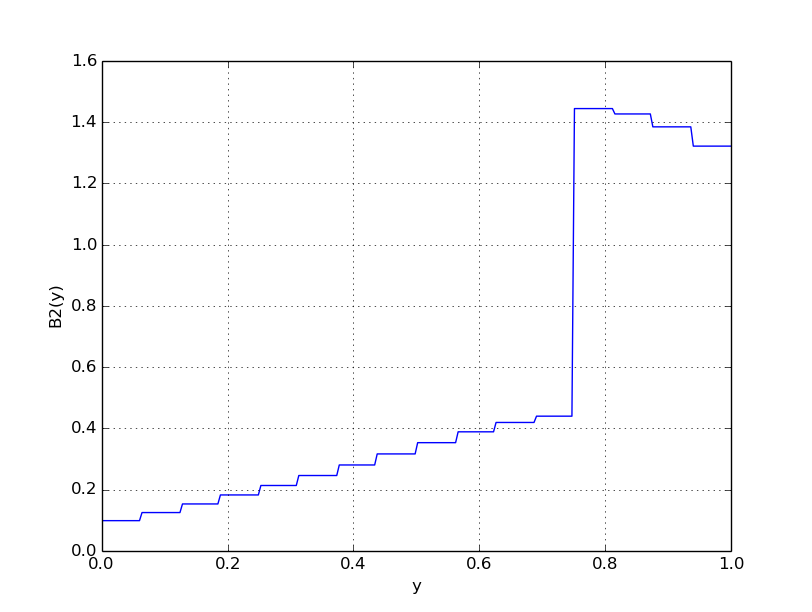
\includegraphics[width=6cm]{f1_025_haar_scale_b2_plot_n_16.png} }}%
    \caption{f1 025 haar scale n 16}%
    \label{fig:f1_025_haar_scale_plot_n_16}%
\end{figure}


\begin{figure}%
    \centering
    \subfloat[f1 025 llmw scale b1 plot n 16]{{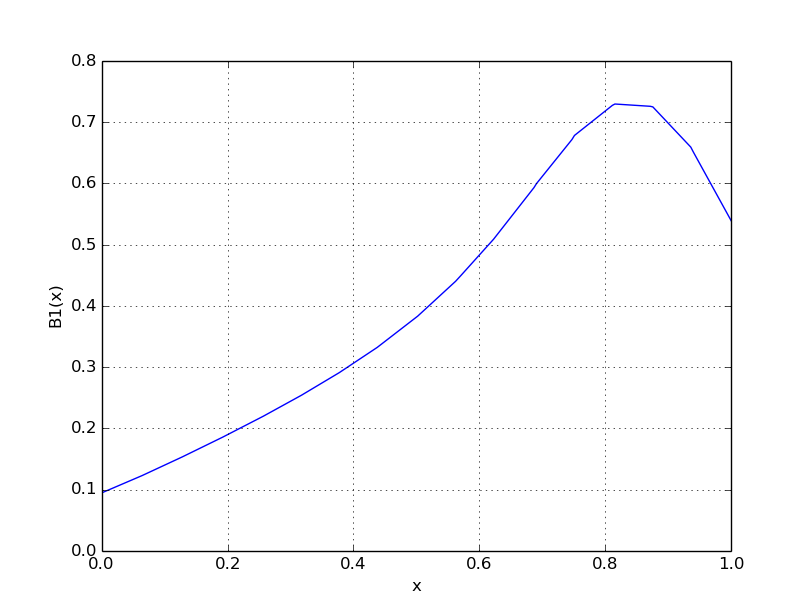
\includegraphics[width=6cm]{f1_025_llmw_scale_b1_plot_n_16.png} }}%
    \qquad
    \subfloat[f1 025 llmw scale b2 plot n 16]{{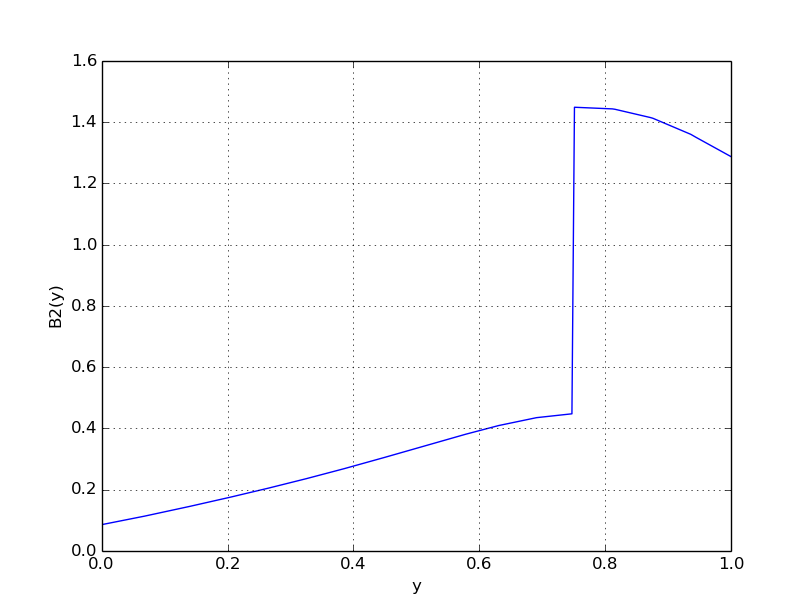
\includegraphics[width=6cm]{f1_025_llmw_scale_b2_plot_n_16.png} }}%
    \caption{f1 025 llmw scale n 16}%
    \label{fig:f1_025_llmw_scale_plot_n_16}%
\end{figure}


\begin{figure}%
    \centering
    \subfloat[f1 025 qlmw scale b1 plot n 16]{{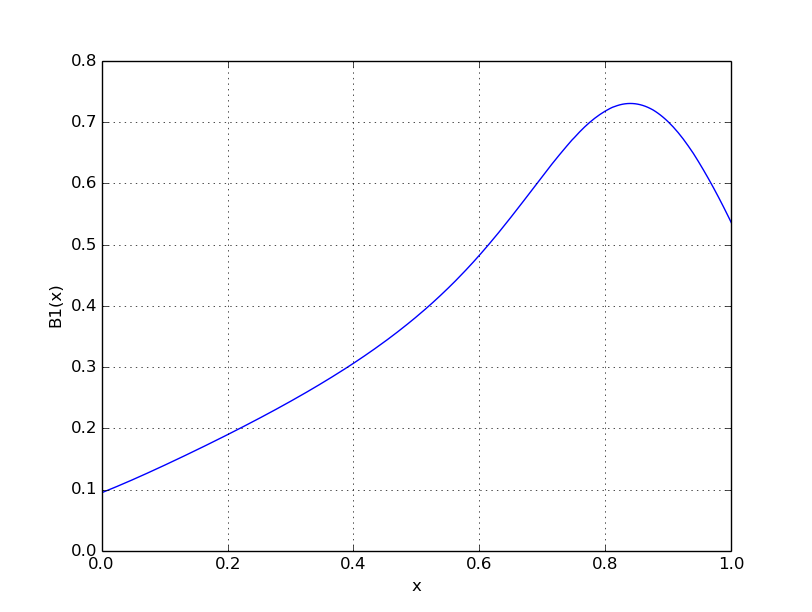
\includegraphics[width=6cm]{f1_025_qlmw_scale_b1_plot_n_16.png} }}%
    \qquad
    \subfloat[f1 025 qlmw scale b2 plot n 16]{{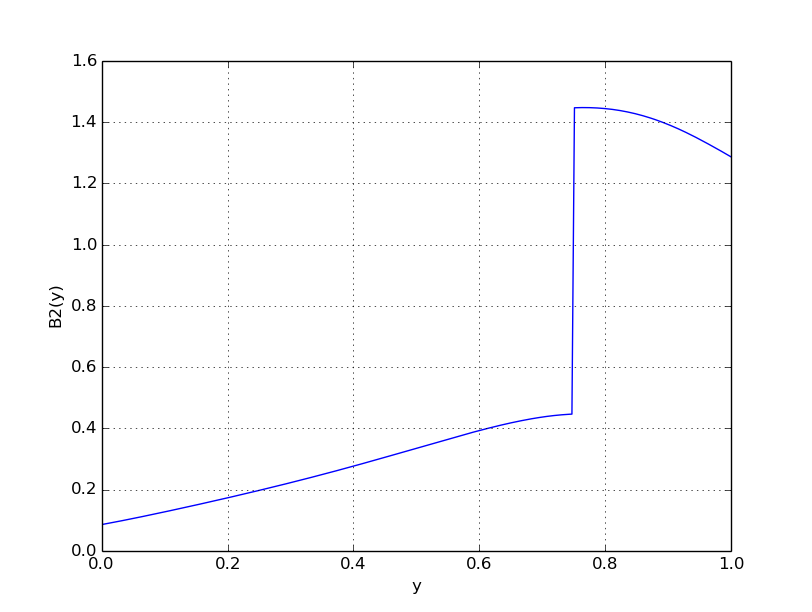
\includegraphics[width=6cm]{f1_025_qlmw_scale_b2_plot_n_16.png} }}%
    \caption{f1 025 qlmw scale n 16}%
    \label{fig:f1_025_qlmw_scale_plot_n_16}%
\end{figure}






\section{Three Dimensional Radiosity}
In this section we show results of projection method to solve 3D radiosity. Scene which we chose is, similar to Flatland scene 1, two square surface aligned and parallel to each other with light source on one of the surface as shown in Figure \ref{fig:3dparallel}. we divided each surface into grid of  $n*n$  sub-square elements of equal size and assumed the radiosity function, over the domain of surface, to be piecewise polynomial over each element. Thus we have projected radiosity function into space spanned by dilates and translates of two dimensional Wavelet basis. We use projection method discussed in Chapter \ref{ch:waveletprojection} to get system of linear equations which are solved to find the unknown projected function. Figure \ref{fig:3dhaar4},\ref{fig:3dhaar4} shows the solution and images of the scene for Haar wavelet with $n=4,16$. Similar to Haar wavelet we can use LLMW and QLMW for projection methods. In case of LLMW we are dealing with space of piecewise linear functions and LLMW wavelet forms the basis for the same space. In case of QLMW, we are dealing with space of piecewise quadratic function for which QLMW wavelet serves as alternative basis. See Figure \ref{fig:3dllmw4},\ref{fig:3dllmw16},\ref{fig:3dqlmw4}.
% Use of this alternative basis give us advantage of sparse matrix for which matrix inversion is faster. Figure \ref{}




\begin{figure}[tbh]
\centering{}
\captionsetup{justification=centering}
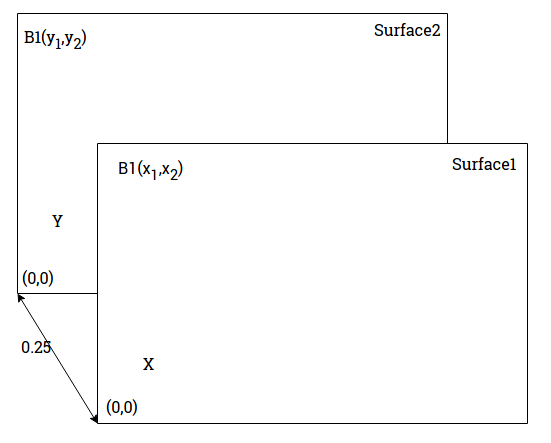
\includegraphics[width=5in]{3dparallel.png}
\caption{\label{fig:3dparallel}3D scene: Two parallel surfaces}
\end{figure}



\begin{figure*}
\centering
\subfloat[Image of Surface 1]{
\includegraphics[width=3in]{3dhaar4_025_1.png}
% \label{fig:llmwphi0}
}\subfloat[Image of Surface 2: With light source at center]{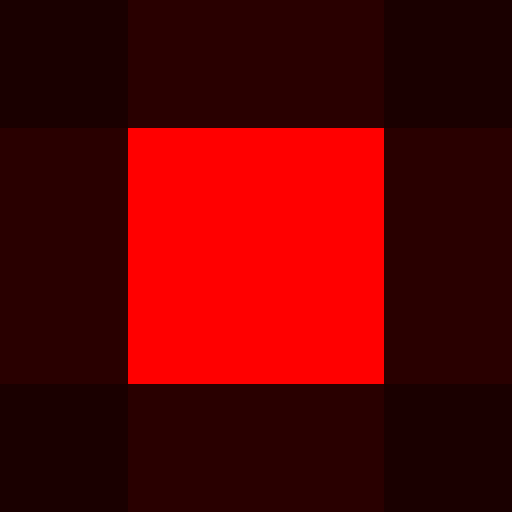
\includegraphics[width=3in]{3dhaar4_025_2.png}
% \label{fig:llmwphi1}
}\\
\caption{\label{fig:3dhaar4}Solution of 3D scene with Haar wavelet and $n=4$}
\end{figure*}


\begin{figure*}
\centering
\subfloat[Image of Surface 1]{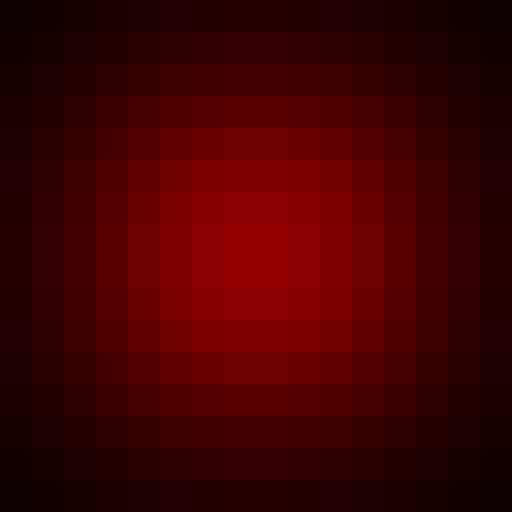
\includegraphics[width=3in]{3dhaar16_025_1.png}
% \label{fig:llmwphi0}
}\subfloat[Image of Surface 2: With light source at center]{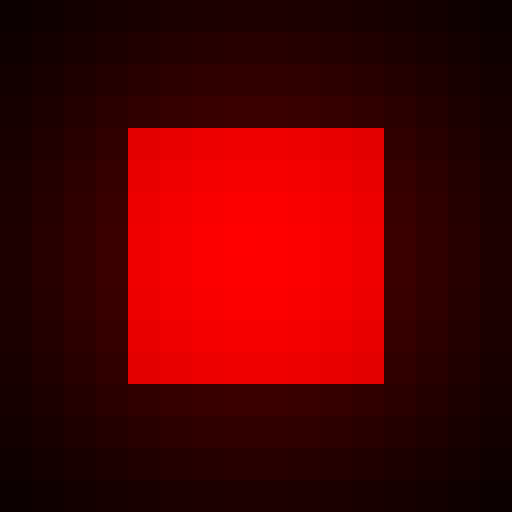
\includegraphics[width=3in]{3dhaar16_025_2.png}
% \label{fig:llmwphi1}
}\\
\caption{\label{fig:3dhaar16}Solution of 3D scene with Haar wavelet and $n=16$}
\end{figure*}



\begin{figure*}
\centering
\subfloat[Image of Surface 1]{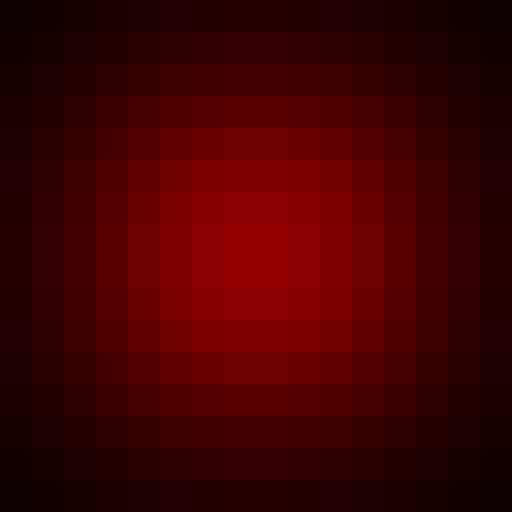
\includegraphics[width=3in]{3dhaar16_025_1.png}
% \label{fig:llmwphi0}
}\subfloat[Image of Surface 2: With light source at center]{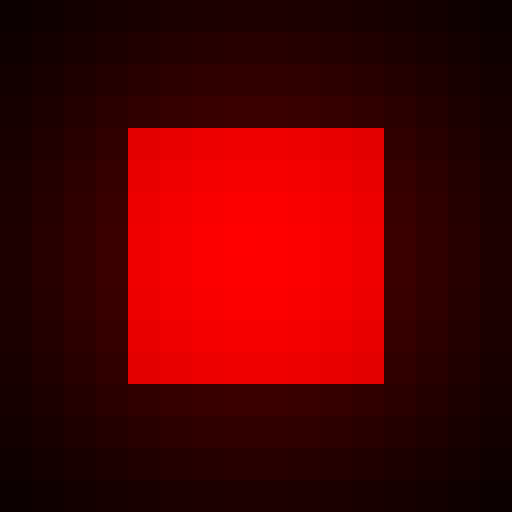
\includegraphics[width=3in]{3dhaar16_025_2.png}
% \label{fig:llmwphi1}
}\\
\caption{\label{fig:3dhaar16}Solution of 3D scene with Haar wavelet and $n=16$, retaining only half of the $256$ coefficients}
\end{figure*}





\begin{figure*}
\centering
\subfloat[Image of Surface 1]{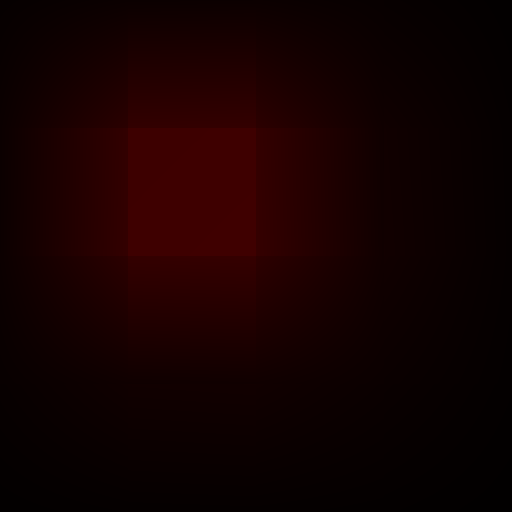
\includegraphics[width=3in]{3dllmw4_025_1.png}
% \label{fig:llmwphi0}
}\subfloat[Image of Surface 2: With light source at center]{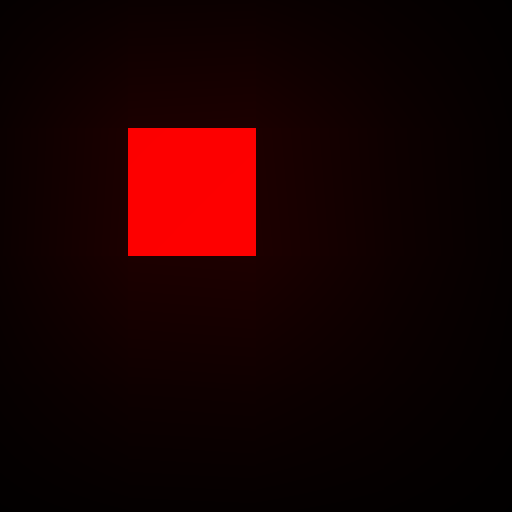
\includegraphics[width=3in]{3dllmw4_025_2.png}
% \label{fig:llmwphi1}
}\\
\caption{\label{fig:3dllmw4}Solution of 3D scene with LLMW wavelet and $n=4$}
\end{figure*}


\begin{figure*}
\centering
\subfloat[Image of Surface 1]{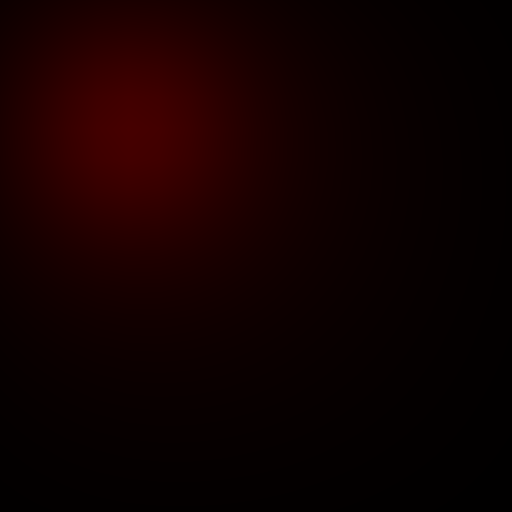
\includegraphics[width=3in]{3dllmw16_025_1.png}
% \label{fig:llmwphi0}
}\subfloat[Image of Surface 2: With light source at center]{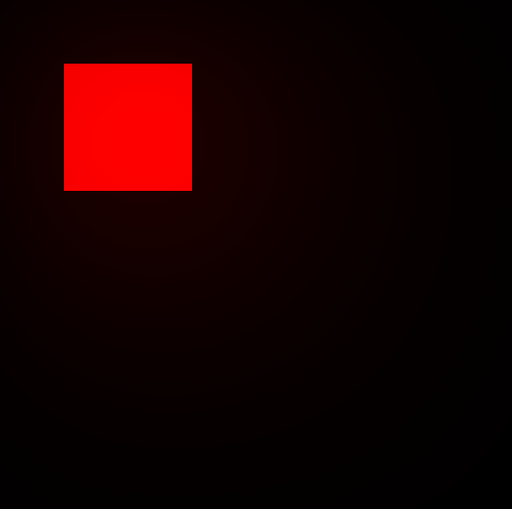
\includegraphics[width=3in]{3dllmw16_025_2.png}
% \label{fig:llmwphi1}
}\\
\caption{\label{fig:3dllmw16}Solution of 3D scene with LLMW wavelet and $n=16$}
\end{figure*}
\begin{figure*}
\centering
\subfloat[Image of Surface 1]{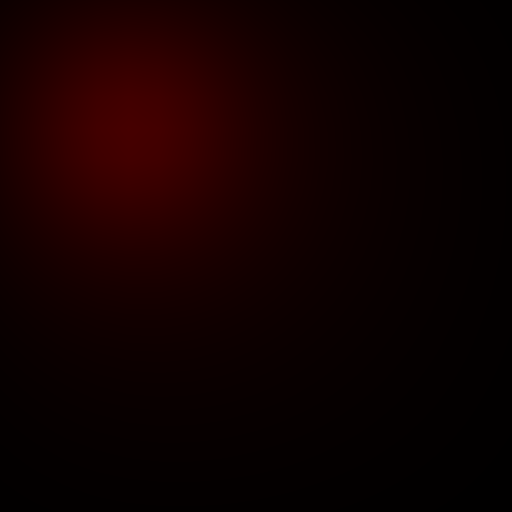
\includegraphics[width=3in]{3dllmw16_025_1.png}
% \label{fig:llmwphi0}
}\subfloat[Image of Surface 2: With light source at center]{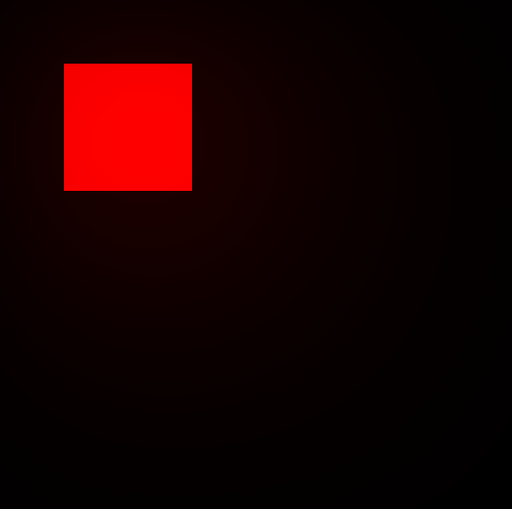
\includegraphics[width=3in]{3dllmw16_025_2.png}
% \label{fig:llmwphi1}
}\\
\caption{\label{fig:3dllmw16}Solution of 3D scene with LLMW wavelet and $n=16$, retaining only quarter of the $1024$ coefficients}
\end{figure*}

\begin{figure*}
\centering
\subfloat[Image of Surface 1]{
\includegraphics[width=3in]{3dqlmw4_025_1.png}
% \label{fig:qlmwphi0}
}\subfloat[Image of Surface 2: With light source at center]{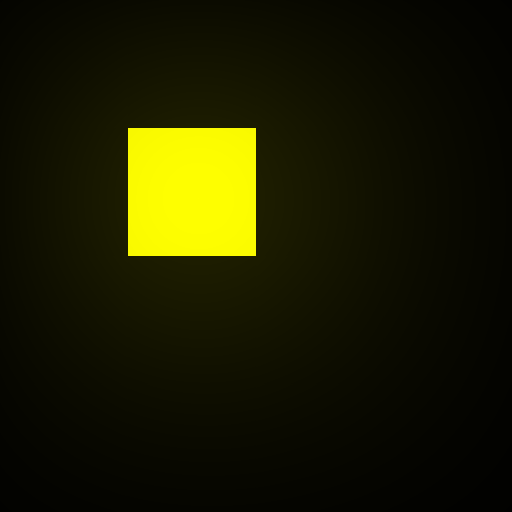
\includegraphics[width=3in]{3dqlmw4_025_2.png}
% \label{fig:qlmwphi1}
}\\
\caption{\label{fig:3dqlmw4}Solution of 3D scene with QLMW wavelet and $n=4$}
\end{figure*}



\begin{figure*}
\centering
\subfloat[Image of Surface 1]{
\includegraphics[width=3in]{3dqlmw4_025_1.png}
% \label{fig:qlmwphi0}
}\subfloat[Image of Surface 2: With light source at center]{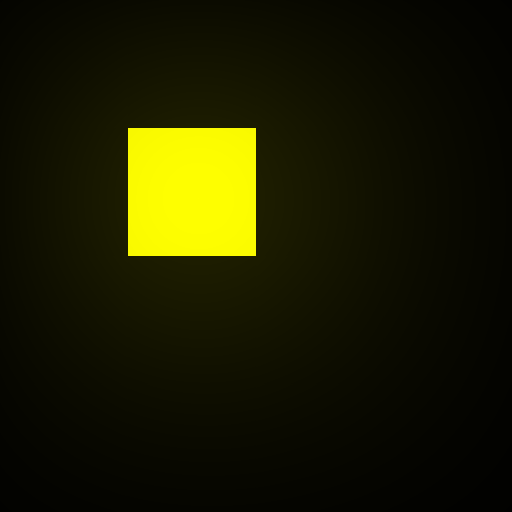
\includegraphics[width=3in]{3dqlmw4_025_2.png}
% \label{fig:qlmwphi1}
}\\
\caption{\label{fig:3dqlmw4}Solution of 3D scene with QLMW wavelet and $n=4$, retaining only half of the $144$ coefficients}
\end{figure*}

% .\\\\\\\\\\\\{\bf flatland}\\

% {\bf 4d}\\
% \\section{Radiosity in three dimension} % (fold)
% \label{sec:radiosity_in_three_dimension}
% \underline{solution and threshold solution}
% % section radiosity_in_three_dimension (end)
